\section{Arquitectura del sistema (\textit{pipeline})}
Aquest apartat descriu l'arquitectura del sistema que s'ha desenvolupat per a l'anàlisi automàtica dels tiquets d'incidències de ciberseguretat de l'\textbf{Agència}. L'arquitectura del sistema està directament lligat a les màquines des de les quals s'han disposat propietat de l'\textbf{Agència} i al sistema que tenien en producció. L'\textbf{Agència} va posar a disposició de l'equip tres servidors idèntics per cada secció on estaran les dades i dos portàtils amb accés als servidors a través d'una VPN privada.

\begin{itemize}
     \item \textbf{Servidor 1 (\textit{OTRS}):} Servidor on s'emmagatzema la base de dades d'\textit{OTRS} amb els tiquets al seu interior.
     \item \textbf{Servidor 2 (\textit{Pipeline}):} Servidor encarregat d'accedir als altres servidors per llegir i guardar informació i passar-la pel programa desenvolupat per resoldre el problema.
     \item \textbf{Servidor 3 (Elasticsearch):} Servidor que recull les dades processades i anonimitzades per un futur us.
\end{itemize}

\begin{itemize}
     \item \textbf{Portàtil 1 (amb GPU):} Portàtil amb la funció principal d'entrenar el model que serà utilitzat per extreure l'informació dels tiquets. Està configurat per evitar cap bretxa de dades.
     \item \textbf{Portàtil 2 (sense GPU):} Portàtil amb la capacitat d'accedir als servidors de l'\textbf{Agència} mitjançant una VPN. Té la mateixa configuració que el Portàtil 1.
\end{itemize}

\begin{figure}[H]
     \centering
     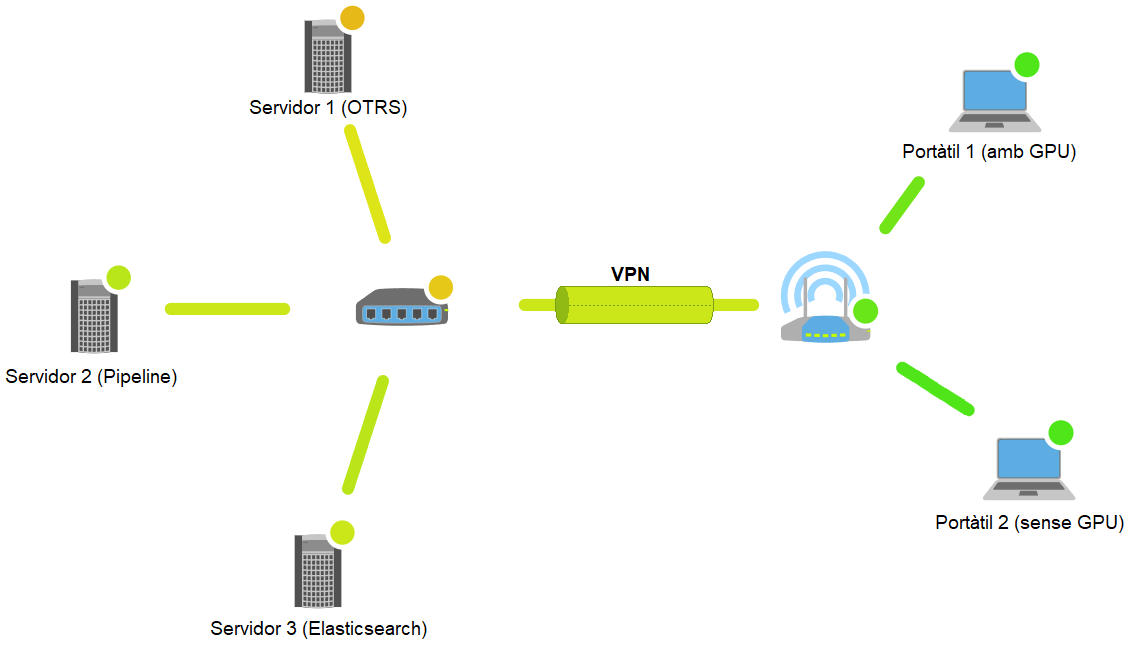
\includegraphics[width=0.8\textwidth]{network.png}
     \caption[Diagrama de la xarxa del projecte]{Diagrama de la xarxa del projecte. \\ (Creació pròpia amb recursos de \textbf{yWorks})}
     \label{fig:network}
\end{figure}

El sistema consta d'una sèrie de scripts de Python que s'executen seqüencialment i duen a terme les tasques següents:

\begin{enumerate}
     \item Extreure els tiquets de la base de dades \textit{OTRS} de l'\textbf{Agència}.
     \item Preprocessar el text de cada tiquet, eliminant el soroll (dades repetides o innecessàries), normalitzant el format i inserint les referències necessàries.
     \item Aplicar un model de processament del llenguatge natural (NLP) que detecta i extreu els camps rellevants de cada tiquet.
     \item Anonimitzar els camps extrets mitjançant una funció a Elasticsearch, que substitueix les dades de sortida per símbols o etiquetes genèriques.
     \item Emmagatzemar els camps anonimitzats en una base de dades Elasticsearch, que és un motor de cerca i anàlisi distribuïda.
\end{enumerate}

La figura \ref{fig:pipeline} mostra un diagrama que il·lustra el funcionament del sistema.

\begin{figure}[H]
     \centering
     \vspace{1cm} % Adjust the vertical space (padding) at the top
     \setlength{\fboxsep}{5pt} % Adjust the padding
     \setlength{\fboxrule}{0pt} % Adjust the border thickness   
     \fbox{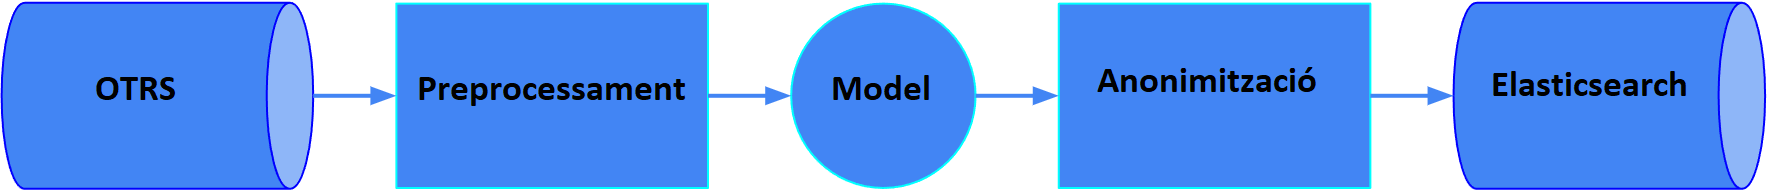
\includegraphics[width=0.8\textwidth]{pipeline.png}}
     \caption[Diagrama de l'arquitectura del sistema]{Diagrama de l'arquitectura del sistema. \\ (Creació pròpia)}
     \label{fig:pipeline}
\end{figure}

En les següents seccions es detallen els components i les tecnologies que han sigut utilitzades a cadascuna de les etapes del \textit{pipeline}.
\subsection{Extracció de tiquets d'OTRS}
% Explicar com està configurat el \textit{OTRS}
Per extreure els tiquets del Servidor \textit{OTRS} de l'\textbf{Agència}, s'ha fa servir \textit{PyOTRS}, que permet accedir a les dades mitjançant peticions a través de la REST API. S'ha implementat un script de Python que utilitza la llibreria mencionada per fer les peticions i obtenir els tiquets. L'script s'encarrega d'autenticar-se amb les credencials cedides per l'\textbf{Agència}, extreure els tiquets especificats a un fitxer Excel i fer un postprocessament per aconseguir tota la informació del tiquet en un format estandarditzat i sense repeticions innecessàries. A continuació es detalla el funcionament del codi seguint l'ordre que recorren els tiquets.

\begin{enumerate}
     \item \textbf{Iniciar sessió:} Es fan unes configuracions per assegurar que els tiquets es reben amb el format esperat i mitjançant les funcions creades a \textit{OTRS}. Després es crea un client amb l'adreça IP del servidor, l'usuari i la contrasenya obtingudes de l'\textbf{Agència}.
     \item \textbf{Iterar pels tiquets:} En cas que s'extreguin molts tiquets seguits es busca i s'obre el fitxer Excel especificat en el qual hi haurà la informació necessària dels tiquets que s'ha de processar. S'itera per la columna en la qual es troben els identificadors dels tiquets. També hi ha una opció per especificar un sol identificador de tiquet.
     \item \textbf{Llegir ID del tiquet:} Per cada fila, es llegeix l'identificador del tiquet i es crida a la següent funció.
     \item \textbf{Comprovar la utilització del tiquet:} Abans de començar a extreure els tiquets, es comprova si el tiquet en qüestió ja ha sigut extret abans. Això es fa per evitar cicles infinits amb referències cícliques dins dels tiquets. Es reinicia la llista de tiquets visitats després de cada iteració.
     \item \textbf{Extreure tiquet:} S'envia la petició al servidor \textit{OTRS} mitjançant la funció \linebreak \pyth{get_ticket_by_number} de \textbf{PyOTRS}. El qual retorna un tiquet de la classe \pyth{Ticket}, molt convenientment, pel seu futur processament. En cas que el tiquet amb l'identificador especificat no existeixi, es llançarà un error informant del succés.
\end{enumerate}


\subsection{Preprocessament de tiquets}
El preprocessament dels tiquets té com a objectiu preparar el text per ser analitzat pel model de NLP. S'ha implementat un script de Python que efectua les operacions següents sobre el text de cada tiquet:
% Com s'organitza el tiquet amb els tres anteriors apartats (posar imatge/exemple)
\begin{enumerate}
     \item \textbf{Iterar pels articles:} El processament bàsic del tiquet consisteix a iterar per tots els articles del tiquet i, per cadascun d'ells unir el cos principal de l'article amb els arxius adjunts i les referències a altres tiquets. Fent això repetit per cada article fins a arribar a l'últim i evitant sempre repetir text ja mencionat anteriorment.
     \item \textbf{Processament del cos:} El primer que s'insereix és el cos principal de l'article que s'està tractant en el moment. Gràcies a una opció d'\textit{OTRS}, el cos està adjuntat com un fitxer adjunt més en format HTML, permetent molta més flexibilitat a l'hora de modificar el seu contingut. Un problema que es va trobar en tots els tiquets, és que per cada article que es contesta, es torna a enviar tota la conversa fins al moment a sota. És per això que es busca l'element HTML que marca el final del tiquet (Una vora esquerra blava) i s'elimina tot el que hi ha dins. Després es converteix a text normal, s'elimina la firma (indica l'hora, lloc i altra informació irrellevant) amb una expressió regular (regex) i s'elimina tots els salts de línia sobrants.
     \item \textbf{Processament dels adjunts:} Els fitxers adjunts estan tots codificats amb la codificació \textbf{Base 64}, per tant, el primer pas és descodificar el fitxer. Després depenent del seu format es fa ús de llibreries diferents per acabar amb el fitxer en format text UTF-8. No tots els fitxers poden ser processats per extreure la seva informació, per exemple, s'ha considerat que analitzar les imatges està fora de l'àmbit d'aquest projecte i, per tant, s'ha decidit tractar els seguents formats:
          \begin{itemize}
               \item \textbf{Fitxer de text (.txt):} Per tractar els fitxers de text, simplement es pot descodificar l'arxiu amb la codificació \textbf{Base 64} i codificar el resultat binari amb la codificació UTF-8.
               \item \textbf{Fitxer de correu electrònic (.msg):} Per processar els fitxers de correu electrònic, s'ha implementat una funció que extreu el contingut de l'adjunt codificat i es descodifica a partir de la codificació \textbf{Base 64}. Les dades binàries després es codifiquen com un missatge d'Outlook amb la llibreria \pyth{extract_msg}. Amb aquest format, ara es pot llegir en format text el remitent, destinatari, subjecte i cos per recrear el correu original.
               \item \textbf{Fitxer PDF (.pdf):} Per llegir fitxers PDF, es descodifica el fitxer codificat a \textbf{Base 64} que representa un arxiu PDF i extreu el contingut de text del PDF descodificat utilitzant una biblioteca de lectura de PDF anomenada \pyth{PyPDF2}. El text extret de cada pàgina es concatena i es torna.
               \item \textbf{Document de Word (.docx):} Aquesta funció descodifica l'adjunt amb la codificació \textbf{Base 64}. El document després es descodifica en dades binàries i fa ús de la llibreria de Python \pyth{docx} per carregar el fitxer .docx des de l'objecte binari. El contingut del document es pot accedir per paràgrafs i es retorna concatenant-los tots.
               \item \textbf{Antic document de Word (.doc):} Per extraure el contingut del document adjunt, el descodifica fent servir la codificació \textbf{Base 64}. Les dades binàries descodificades s'escriuen en un fitxer temporal amb extensió .doc. Després, s'utilitza l'eina externa \pyth{antiword} a través d'un subprocés per convertir el fitxer temporal .doc en text pla. Finalment, es torna el text extret com a resultat de la funció.
          \end{itemize}
     \item \textbf{Processament de les referències:} Aquesta funció intenta buscar en el text totes aquelles referències a incidències passades per intentar recrear tot el context necessari per entendre el tiquet. Es defineix un patró d'expressió regular que cerca exactament 16 dígits, que representen un número de tiquet, i cerca totes les aparicions d'aquest patró dins de l'article. Per a cada número de tiquet identificat, es recupera informació detallada sobre el tiquet referenciat utilitzant la funció \pyth{get_ticket_by_number} i indicant, en cas que sigui necessari si ja ha sigut inserida aquesta referència anteriorment.
     \item \textbf{Unir i retornar:} Finalment, s'uneixen totes les peces en un mateix text, de manera que quedarien els articles ordenats temporalment i, sota de cada article, el text dels fitxers adjunts (si han pogut ser descodificats) i els tiquets als quals es fan referència.
\end{enumerate}

\subsection{Eliminació de signatures i peus de pàgina}
La majoria dels articles d'un tiquet contenien un últim paràgraf que contenia informació genèrica sobre ciberseguretat, telèfons o correus de contacte, advertències, etc. A més a més, a sobre d'aquest peu de pàgina hi havia una signatura automàtica informant de la seva posició a l'empresa, ubicació, etc. 

Combinant les signatures i els peus de pàgina, hi havia articles on la majoria de text era aquesta part irrellevant del correu. Es va considerar que aquesta informació no era rellevant per a l'entrenament del model principal, ja que el fet que un correu fos confidencial o el número de telèfon d'una persona no hauria d'influir en el resultat, pel fet que no era cap dels camps que es buscava extreure. L'objectiu d'aquest model de "preprocessament" dels articles era:

\begin{itemize}
     \item Alleugerir la càrrega computacional del model principal.
     \item Mostrar al model només la informació rellevant.
     \item Permetre entrenar amb més informació d'entrada com els adjunts dels tiquets o les referències.
\end{itemize}

Per a l'entrenament d'aquest model es va decidir treballar amb articles individuals en comptes de amb tot el tiquet, ja que les signatures són individuals de cada article i no en general al tiquet. Això també va permetre la possibilitat d'utilitzar models amb un context més reduït.

\subsubsection{Conjunt de dades}
L'objectiu del model és rebre el text d'un article directament com surten del procés de preprocessament de tiquets i obtenir com a resultat un tiquet sense les signatures ni peus de pàgina mencionats anteriorment. S'ha plantejat diverses maneres en què un model pot aprendre aquest comportament desitjat:

\begin{itemize}
     \item \textbf{Detectar el text:} El resultat d'aquest model és directament el text rellevant que es vol. No és necessari cap processament després d'obtenir el resultat.
     \item \textbf{Detectar la signatura:} El resultat del model serà la signatura present a l'article, en cas que no n'hi hagi cap, no es retornaria res. Després es pot detectar aquesta signatura en l'article d'entrada i eliminar-la. El problema que presenta aquest mètode és que en cas que el model escrigui una sola lletra incorrectament del resultat ja no es podria trobar al text original.
     \item \textbf{Detectar caràcter d'inici de la signatura:} S'ha vist que la majoria de les correccions que es poden realitzar a un article es troben al final. Aprofitant aquest fet, es pot entrenar un model que indiqui a partir de quina alçada s'inicia la signatura i així poder-la retallar. No obstant hi ha casos on informació rellevant com el departament de la persona que escriu l'article pot ser esborrat.
     \item \textbf{Classificació de frases:} Inspirat en altres projectes amb objectius similars, s'ha plantejat un conjunt de dades amb elements més reduïts i simples en forma de frase i que l'objectiu sigui classificar-les segons si formen part de la signatura o no. Utilitzant un altre model del llenguatge natural, es pot dividir un text en frases i, reutilitzant intel·ligentment les dades dels conjunts de dades anteriors, es pot evitar tornar a etiquetar. Per tenir més flexibilitat, s'ha afegit la posició de la frase dins de l'article juntament amb el nombre de frases totals de l'article. Totes aquestes dades ens poden ajudar a classificar millor si una frase pertany a una signatura.
\end{itemize}

\subsubsection{Entrenament}
A continuació es presenten els models utilitzats i quin ha sigut el conjunt de dades en el que s'ha entrenat.

\underline{Flan-T5-Base}

Aquest model s'ha entrenat amb l'objectiu de detectar el text dels articles, descartant en el procés les signatures. Utilitzant les tècniques de Gradient Checkpointing i Gradient Accumulation, s'ha aconseguit entrenar aquest model dins de la GPU de 8GB sacrificant en el procés el temps d'entrenament. S'ha entrenat durant 10 epochs que ha sigut l'equivalent a més de 24 hores d'entrenament continuat.
Tot i el bon historial d'aquest model, el resultat d'aquest \textit{fine-tuning} ha sigut un fracàs. El model no ha sigut capaç de generalitzar la tasca d'eliminar la signatura, ni en els casos on més es repetia. La causa d'aquest mal entrenament queda desconeguda, ja que aquesta tasca es considera teòricament senzilla de resoldre per un model del llenguatge natural.

\underline{FLOR-760M}

A causa del fet que el model \textbf{Flan-T5-Base} no va demostrar bons resultats en eliminar les signatures dels correus, es va decidir canviar de model. El model \textbf{FLOR} és un model de llenguatge causal basat en l'arquitectura \texttt{Transformers} per a català, castellà i anglès. És el resultat d'una tècnica d'adaptació lingüística realitzada al model \textbf{BLOOM}, que implica modificar el vocabulari del model i la capa d'\textit{embedding}, i entrenar el model contínuament amb 26B \textit{tokens} en les llengües mencionades. S'ha escollit el model de 760M i s'ha fet l'entrenament per 5 \textit{epochs}.
En observar els resultats de l'entrenament, s'esperaven resultats acceptables pel nostre cas d'ús. Això no obstant, en fer l'avaluació en les dades de test, hem vist que el model no generalitza bé. Addicionalment, un altre desavantatge del model és el temps d'inferència. Es va veure que en netejar un article tarda entorn d'un minut, la qual cosa fa inviable netejar les dades amb un model de generació de text.
A causa d'aquests problemes, s'ha decidit canviar el conjunt de dades i, en conseqüència, el mètode per detectar les signatures en els articles dels tiquets.

\underline{Modificació RoBERTa}

Com que els models generatius triguen molt a executar-se i no s'havia trobat resultats bons amb els models provats, es va decidir canviar de mètode per resoldre el problema. Es va canviar el problema d'un problema de generació de text a un problema de classificació de frases. Per a classificar les frases el que es vol aconseguir és convertir cada frase en un vector de mida fixa que respresenti el significat de la frase i utilitzar-lo per classificar-la com a una de les dues classes resultat: "pertany a una signatura" o "no pertany a una signatura". Per a fer-ho, s'ha fet servir el model \textbf{RoBERTa} per a generar un \textit{embedding} de la frase i s'ha emprat una sèrie de capes denses que reben aquest vector i el processen iterativament fins a arribar a una capa de classificació amb dues neurones on la neurona més activada indica quina classe ha sigut escollida.
Addicionalment, s'ha afegit una capa que donada la posició de la frase i el nombre de frases per arribar al final (ambdues normalitzades entre 0 i 1), augmenta la seva mida fins a arribar a la mateixa que els \textit{embeddings}, així tenen una representació igual i no són menyspreats. Aquests números es concatenen amb els \textit{embeddings} i es posen com a input a les capes de classificació per a aconseguir més informació sobre la frase.
Després de moltes iteracions (més de 10) sobre l'arquitectura del model, la naturalesa de les dades i la manera d'entrenament, s'ha arribat a la conclusió que la millor precisió a la qual pot arribar és a un 87\%. Això significa que només un 87\% de les frases seran classificades correctament, obtenint potencialment un correu que perd molta informació que pot ser vital per comprendre la incidència o trobar alguns camps. És per això que no es considera que aquest model es pugui utilitzar en producció i es continua fent recerca per resoldre aquest problema.

\underline{Spacy Pipeline}

Els últims resultats amb el model \textbf{RoBERTa} van deixar veure que una classificació incorrecta pot causar perdre informació important d'un tiquet. És per això que provar un últim mètode utilitzant el mateix conjunt de dades. Es va decidir implementar una solució més tradicional fent servir la llibreria \textit{Spacy}.
\textit{Spacy} és una llibreria de processament del llenguatge natural desenvolupada en Python que ofereix eines eficients per analitzar i processar text de manera precisa i eficaç. Amb \textit{Spacy}, es pot acomplir diverses tasques de NLP, com ara etiquetar de manera automàtica el tipus de paraules en un text (\textit{POS tagging}), reconeixement d'entitats, anàlisi de dependències sintàctiques, etc. Una de les funcionalitats destacades de \textit{Spacy} és la seva capacitat per a la classificació de textos, que permet etiquetar automàticament els documents o fragments de text en categories prèviament definides.
Es va fer servir la \textit{pipeline} tradicional que fa servir \texttt{tok2vec} en comptes de \texttt{Transformers} per crear els \textit{embeddings} de les frases. S'ha fet servir \texttt{tok2vec}, ja que no requereix GPU pel seu funcionament. En cas que es volgués fer servir \texttt{Transformers} per millorar els resultats, faria falta disminuir la versió de \textit{Cuda toolkit} de 12.1 a 11.8. La causa d'això és el fet que encara hi ha llibreries com \texttt{Cupy} (essencial per entrenar \textit{Spacy} amb models de \texttt{Transformers}) que requereixen la versió \textit{Cuda toolkit} 11.8. Malauradament, són necessaris permisos d'administrador per disminuir la versió i per això es va decidir fer servir CPU amb \textit{Spacy}.
Encara que s'ha fet servir un mètode més tradicional, s'ha millorat els resultats respecte al model de \texttt{Transformers} i s'ha aconseguit una \textit{f1 score} de 90. Es pot observar que els resultats són impressionants considerant que no es fa servir \texttt{Transformers}, un mètode estat de l'art. Si en el futur es considerés que s'hauria de reprendre el model d'eliminació de signatures, es demanaria permís per disminuir la versió de \textit{Cuda toolkit} de 12.1 a 11.8.

\subsubsection{Conclusió eliminació de signatures i peus de pàgina}
En conclusió, el desenvolupament d'un model d'eliminació de signatures eficaç ha estat ple de reptes i contratemps. Els models inicials, inclosos el \textbf{Flan-T5-Base} i el \textbf{FLOR-760M}, no van assolir les expectatives establertes, lluitant amb la generalització i els temps d'inferència poc pràctics. El posterior canvi a la classificació de frases mitjançant el model \textbf{RoBERTa} també va quedar curt, aconseguint una precisió que, tot i que lloable, no era suficient per al desplegament en un entorn de producció a causa del risc d'omissió informació crítica.

L'exploració de mètodes tradicionals amb el \textit{pipeline} \texttt{tok2vec} de \textit{Spacy} ha donat resultats prometedors, superant els dels models \texttt{Transformer} més avançats. Tanmateix, la \textit{f1 score} de 90, tot i ser un assoliment important, no proporciona el nivell de confiança necessari per garantir que no es perdi cap informació important durant el procés d'eliminació de la signatura. Aquesta desconfiança prové del fet que hi ha articles on la informació més rellevant sol estar al final de l'article en una mena de resum fet per la persona que ha resolt el tiquet. La pèrdua d'aquesta informació pot reduir l'efectivitat del model d'extracció posterior. Per tant, s'ha pres la decisió de no utilitzar aquest model en el seu estat actual. A més a més, a causa de les limitacions de temps, l'enfocament s'ha desplaçat cap a la millora del model principal, que és fonamental per al projecte.

\subsection{Aplicació del model}
Per aplicar el model NLP que detecta i extreu els camps rellevants de cada tiquet, s'ha fet servir la llibreria \texttt{Transformers}.

\texttt{Transformers} és una biblioteca de codi obert desenvolupada per \textit{Hugging Face} \cite{Hugging-Face} que ofereix models preentrenats i eines per a tasques de processament del llenguatge natural. Aquesta llibreria facilita molt l'aplicació del model i, després d'instalar totes les dependències requerides, s'utilitza la següent commanda per inicialitzar un \textit{pipeline}, que amaga tot el procés d'inferència:

\begin{python}
t2t_gen_pipe = pipeline(
     "text2text-generation",
     model='./trained_model/',
     tokenizer='google/flan-t5-base',
     device='cuda'
     )     
output_text = t2t_gen_pipe(input_ticket_str, max_new_tokens=300, beams=5)[0]['generated_text']
\end{python}

Aquest codi inicialitza un \textit{pipeline} amb la funció de generació de text a text (la tasca del model \textit{Flan-T5}), el model afinat anteriorment, el \textit{tokenitzador} per defecte del model i s'indica que es faci ús dels drivers de cuda, per aprofitar tota la potència computacional de la GPU. Amb aquest \textit{pipeline}, s'indica l'entrada, el nombre màxim de \textit{tokens} que pot generar el model (el model té la capacitat per parar sol, però s'indica un màxim com a mesura de seguretat) i el nombre de \textit{beams} (possibles solucions candidates, diferents unes de les altres) durant el \textit{beam search}. Aquest mètode es pot aplicar per molts altres models pertanyents al repositori de \textit{Hugging Face}. El que és diferent és com s'ha de preparar les dades per oferir al model el millor format pel seu enteniment.

El model rep com a entrada el text d'un tiquet ja preprocessat en el format específic, i ofereix com a sortida els camps desitjats en format JSON, incloent-hi el valor que ha pogut extreure per a cada camp. En cas que no hagi trobat algun camp, el model retornarà "NotFound". El model ha estat entrenat específicament perquè sempre retorni un JSON. Al ser un model generatiu, es pot donar el cas que no retorni un JSON amb format adequat. No obstant, no s'ha trobat cap cas i la probabilitat que això passi és molt baixa, però cal tenir-ho en consideració. 

Després que el model tregui la sortida i es comprobi que és en un format JSON llegible, s'afegeix en aquesta sortida el nom del tiquet en el camp \textit{file} per donar més flexibilitat en la cerca en el futur. En la figura \ref{fig:format-sortida-dades} es pot veure el format de les dades de sortida.

\begin{figure}[H]
     \centering
     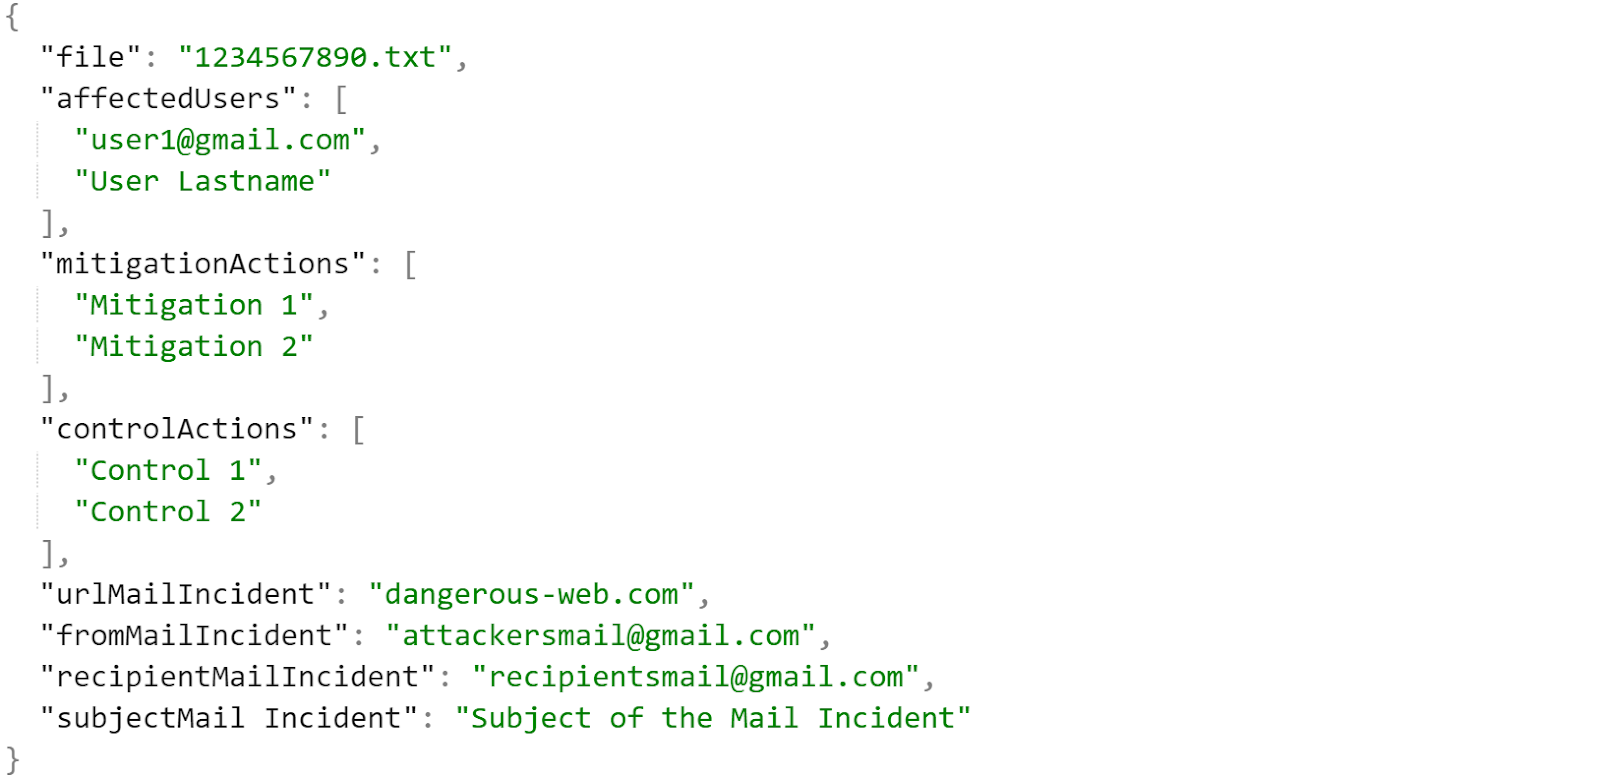
\includegraphics[width=\textwidth]{format_sortida_dades.png}
     \caption[Format de sortida del model]{Exemple d'un tiquet mostrant el format de sortida del model. \\ (Creació pròpia)}
     \label{fig:format-sortida-dades}
 \end{figure}

\subsection{Anonimització de camps}
Per a l'anonimització dels camps l'\textbf{Agència} va demanar fer servir \textit{Logstash} tal com s'explica al blog oficial de la pàgina d'elastic \cite{Logstash}. En aquest blog s'ofereix una guia completa sobre la pseudonimització, una tècnica de protecció de dades recomanada pel Reglament General de Protecció de Dades (GDPR). Explica com la pseudonimització altera les dades personals per impedir que s'atribueixin a una persona concreta sense informació addicional. Es pot diferenciar entre dades pseudònimes, que es poden tornar a identificar amb informació addicional, i dades anònimes.

Es fa servir el mètode proposat per a la pseudonimització de dades durant la ingestió a \textit{Elasticsearch} utilitzant una tècnica d'empremta digital (\textit{fingerprinting}) i \textit{Logstash}, el motor de processament.

La tècnica per aconseguir la pseudonimització consisteix a substituir els camps identificadors per una representació hash i emmagatzemar les dades originals i una clau generada en una base de dades separada, que permeti la reversió futura en cas necessari. Aquesta base de dades separada s'anomena \textit{identity}.

Durant la ingestió de dades a \textit{Elasticsearch}, s'utilitza un filtre \textit{fingerprint} de \textit{Logstash} per realitzar un hash de cada camp que s'emmagatzema a la base de dades. El hash es converteix en les dades pseudonimitzades, sobreescrivint el valor del camp identificador original. Els hash i els valors originals dels camps identificadors s'emmagatzemen per separat als en bases de dades diferents.

La configuració de \textit{Logstash} assumeix una única instància d'\textit{Elasticsearch} que escolta a un port específic. Aquest clúster emmagatzema les dades pseudonimitzades en un índex i els documents \textit{identity} en un altre. La configuració es pot modificar per enviar aquests documents a clústers separats si es requereix un grau més gran de separació.

El hash utilitza una clau especificada a la configuració, la qual cosa proporciona un efecte de \textit{salat} aleatori (afegir caràcters al final de la contrasenya per augmentar la seva robustesa). Es fa servir el mètode SHA-256 per a generar el hash, però l'elecció específica de l'algorisme hash es pot configurar. Addicionalment, també es pot escollir els camps que es vulguin anonimitzar actualitzant un paràmetre de la funció. Tots els camps que no siguin dins del paràmetre (com el nom del fitxer \textit{file}), s'emmagatzemaran sense anonimitzar.

L'identificador de cada entrada és el hash únic associat a l'entrada, cosa que evita la duplicació de dades. Això també permet als administradors consultar els valors de la petjada digital amb una simple cerca d'un identificador.

\subsection{Emmagatzematge del resultat}
A l'etapa final de la cadena de processament dels tiquets, l'\textbf{Agència} ha fet servir \textit{Elasticsearch} com a solució d'emmagatzematge per als camps extrets. \textit{Elasticsearch} és conegut per les seves capacitats de cerca distribuïda i en temps real, cosa que el fa eficient per gestionar i consultar grans volums de dades estructurades.

El procés d'emmagatzematge dels resultats normalment es faria amb una crida a una llibreria específica de \textit{Elasticsearch} de la mateixa a manera que es fa per descarregar els tiquets amb \textit{PyOTRS}, però ara és gestionat per \textit{Logstash}. Amb el \textit{Logstash} configurat, quan es rep un fitxer JSON mitjançant TCP, automàticament anonimitza, distribueix i emmagatzema el resultat en la base de dades \textit{Elasticsearch} especificada.